\documentclass[psamsfonts]{amsart}

%---- MY PACKAGES -----

\usepackage{hyperref}

% Adjust as necessary for sizing
% \usepackage[left=3cm, right=3cm, top=3cm, bottom=3cm]{geometry}

\usepackage{tikz}
\usepackage{circuitikz}
\usetikzlibrary{arrows.meta, positioning}

% Used for in-text code
\usepackage{listings}
\usepackage{xcolor}

\lstset{
  basicstyle=\ttfamily\small,
  backgroundcolor=\color{gray!10},
  frame=single,
  breaklines=true,
  postbreak=\mbox{\textcolor{red}{$\hookrightarrow$}\space},
  keywordstyle=\color{blue},
  commentstyle=\color{gray},
  stringstyle=\color{orange},
  numbers=left,
  numberstyle=\tiny\color{gray}
}

% Used for psuedocode
\usepackage{algorithm}
\usepackage{algpseudocode}  % Extension of algorithmicx
% \algrenewcommand{\algorithmiccomment}[1]{\hfill\(\triangleright\) #1}

% Used to adjust algorithm placement
\usepackage{float}

% For subfigure command
\usepackage{subcaption}


\newcommand{\mycomment}[1]{} 
\usepackage{graphicx} 

%-------THEIR PACKAGES---------
\usepackage{amssymb,amsfonts}
\usepackage[all,arc]{xy}
\usepackage{enumerate}
\usepackage{mathrsfs}

%--------Theorem Environments--------
%theoremstyle{plain} --- default
\newtheorem{thm}{Theorem}[section]
\newtheorem{cor}[thm]{Corollary}
\newtheorem{prop}[thm]{Proposition}
\newtheorem{lem}[thm]{Lemma}
\newtheorem{conj}[thm]{Conjecture}
\newtheorem{quest}[thm]{Question}

\theoremstyle{definition}
\newtheorem{defn}[thm]{Definition}
\newtheorem{defns}[thm]{Definitions}
\newtheorem{con}[thm]{Construction}
\newtheorem{exmp}[thm]{Example}
\newtheorem{exmps}[thm]{Examples}
\newtheorem{notn}[thm]{Notation}
\newtheorem{notns}[thm]{Notations}
\newtheorem{addm}[thm]{Addendum}
\newtheorem{exer}[thm]{Exercise}

\theoremstyle{remark}
\newtheorem{rem}[thm]{Remark}
\newtheorem{rems}[thm]{Remarks}
\newtheorem{warn}[thm]{Warning}
\newtheorem{sch}[thm]{Scholium}

\makeatletter
\let\c@equation\c@thm
\makeatother
\numberwithin{equation}{section}

%--------Meta Data: Fill in your info------
\title{Real-Time Hyperspectral Image Processing \\REU Final Report}

\author{Nash Rickert}

% \date{DEADLINES: Draft AUGUST 15 and Final version AUGUST 29, 2019}

\begin{document}

\begin{abstract}

    Hyperspectral imaging is widely used for environmental monitoring and other tasks, but the processing stage can often take days or weeks which limits the ability of workers to effectively make use of collected data. The goal of our project is to create a system capable of real-time hyperspectral image processing using custom hardware. To this end, I investigated model architectures that can process data efficiently on our system. I discovered that a Kolmogorov-Arnold neural network can be efficiently encoded as lookup tables which approximate the model without a large corresponding drop in accuracy. However, these tables take up an excessive amount of space in the local memory of our system. To resolve this problem, I created a Linux block device driver that can efficiently load large amounts of data to the local memory of our device.


\end{abstract}

\maketitle

\vspace{-1em}

\tableofcontents

% \section{Project Overview}
\section{Hyperspectral Imaging}
While an RGB image samples only the three spectral bands associated with the colors red, green, and blue in the visible spectrum to form an image, a hyperspectral imager uses diffraction to sample a continuous range of spectral bands, including those falling outside of the visible spectrum as shown in \autoref{fig:image2}. This is useful for many tasks such as environmental monitoring because hyperspectral images can account for characteristics of the data that would not exist in an RGB image. For example, the chlorophyll in vegetation absorbs most visible light, but its reflectance changes rapidly near the infrared range of the spectrum. This phenomenon is called the `red edge', and makes identifying vegetation relatively straightforward using hyperspectral imaging. For our project, we are seeking to leverage these advantages to identify forest regions with an abundance of ground fuel to classify areas at risk of forest fires.

\begin{figure}[ht]
  \centering
  \begin{subfigure}[b]{0.37\textwidth}
    \centering
    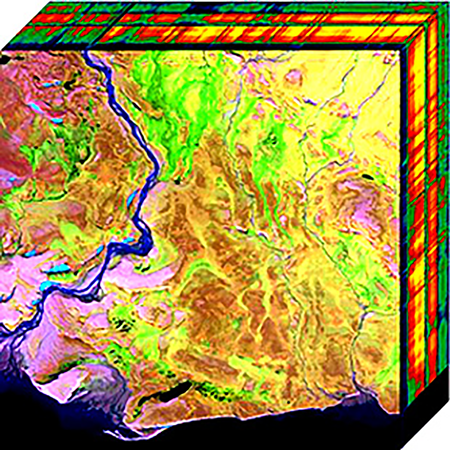
\includegraphics[width=\textwidth]{datacube.png}
    \caption{A hyperspectral data cube \cite{hsi-cube}}
    \label{fig:image1}
  \end{subfigure}
  \hfill
  \begin{subfigure}[b]{0.53\textwidth}
    \centering
    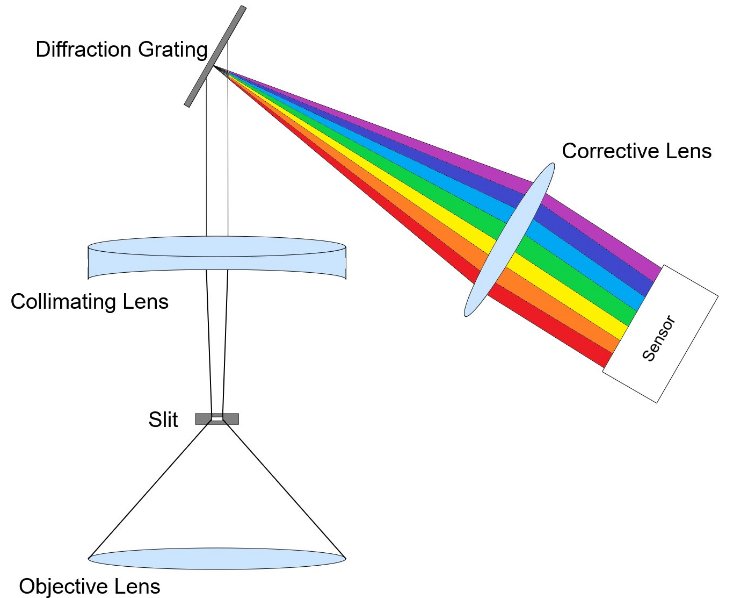
\includegraphics[width=\textwidth]{hsi_optics.png}
    \caption{The optics of a hyperspectral imager \cite{nat-presentation}}
    \label{fig:image2}
  \end{subfigure}
  \caption{The depth of a hyperspectral data cube represents the many color channels that make up each pixel.}
  \label{fig:hsi}
\end{figure}


As a result of the continuous sampling of the spectrum, hyperspectral images contain much more data than a traditional image. The sensor we are using collects data on 1608 color channels compared to the 3 channels of an RGB image. While binning can reduce the number of channels we utilize and the corresponding size of our images, the sheer quantity of hyperspectral data is a major obstacle to its effective analysis.

\section{Real Time Processing}
Traditionally, hyperspectral data is captured in the field and returned to a lab for processing. This process can be lengthy and tedious due to the large size of hyperspectral data -- the data may be many gigabytes or even terabytes in size, meaning the processing stage can take days or weeks.\mycomment{Note: is this true??} For time-sensitive environmental tasks, it would be preferable to process data as the sensor receives it. This would allow field workers to utilize data for decision-making as they receive it and would eliminate the need for persistent storage. For example, when classifying which areas of a forest need to be cleared of ground fuel, workers could fly a drone equipped with a sensor and real-time processor; upon completion, they could immediately begin clearing debris.

Machine learning classification tasks are generally done with GPUs due to their parallelism and efficiency at completing arithmetic operations. For this reason, a strong infrastructure exists for training and running models on a GPU, making their design and implementation relatively easy. Unfortunately, GPUs have several drawbacks that make them unsuitable for our purposes. In the process of completing inference on data received from a sensor, it is necessary for the CPU to write data from the sensor into DRAM, load the data from DRAM into the GPU, perform the inference operation, and then finally write results back to DRAM as shown in \autoref{fig:gpu-diagram}. The overhead of writing and loading the data and writing the results back to DRAM is inordinate when our goal is to complete inference at the same rate that data is received. Furthermore, cache misses and refresh rates make the processing speed of a GPU nondeterministic and unpredicatble, and the weight and power-consumption of a GPU would be difficult to accommodate on a drone. Thus we choose to use a field-programmable gate array (FPGA) for our project. An FPGA has the advantage that data can be streamed in directly from the sensor and pipelined deterministically through the fabric of our circuit as shown in \autoref{fig:fpgadiagram}. Therefore, the main challenge of this project is to effectively leverage the advantages of custom hardware to achieve rapid inference. While potentially advantageous, this entails many more difficulties and pitfalls than one would typically encounter when using a GPU.
% Don't just forshadow, give examples. Such as efficiently pipelining, small amount of static ram, etc. (literally have to program the damn thing)


% CPU/GPU processing diagram
\begin{figure}[ht]
  \centering
  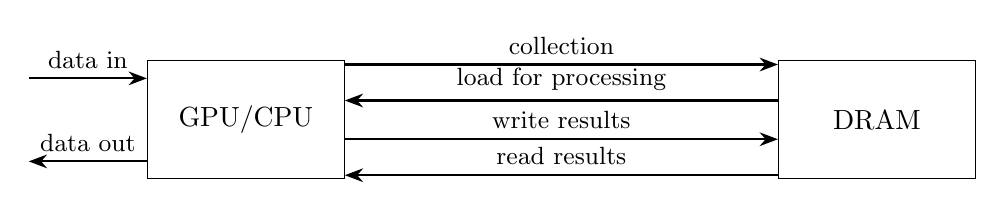
\begin{tikzpicture}[
    block/.style={rectangle, draw, minimum width=2.5cm, minimum height=1.5cm, align=center},
    arrow/.style={-{Stealth}, thick},
    textnode/.style={font=\small}
    ]

    % Nodes
    \node[block] (gpu) {GPU/CPU};
    \node[block, right=5.5cm of gpu] (dram) {DRAM};

    \coordinate[left=1.5cm of gpu.west, yshift=15pt] (datain);
    \coordinate[left=1.5cm of gpu.west, yshift=-15pt] (dataout);

    % Data in and out arrows
    \draw[arrow] (datain) -- ([yshift=15pt]gpu.west) node[midway, above, textnode] {data in};
    \draw[arrow] ([yshift=-15pt]gpu.west) -- (dataout) node[midway, above, textnode] {data out};


    % Spaced arrows between GPU and DRAM (top to bottom)
    \draw[arrow] ([yshift=20pt]gpu.east) -- ([yshift=20pt]dram.west) node[midway, above, textnode] {collection};
    \draw[arrow] ([yshift=7pt]dram.west) -- ([yshift=7pt]gpu.east) node[midway, above, textnode] {load for processing};
    \draw[arrow] ([yshift=-7pt]gpu.east) -- ([yshift=-7pt]dram.west) node[midway, above, textnode] {write results};
    \draw[arrow] ([yshift=-20pt]dram.west) -- ([yshift=-20pt]gpu.east) node[midway, above, textnode] {read results};

  \end{tikzpicture}
  \caption{Latency overhead of using a GPU for computation}
  \label{fig:gpu-diagram}
\end{figure}

% FPGA Data stream diagram
\begin{figure}[ht]
  \centering
  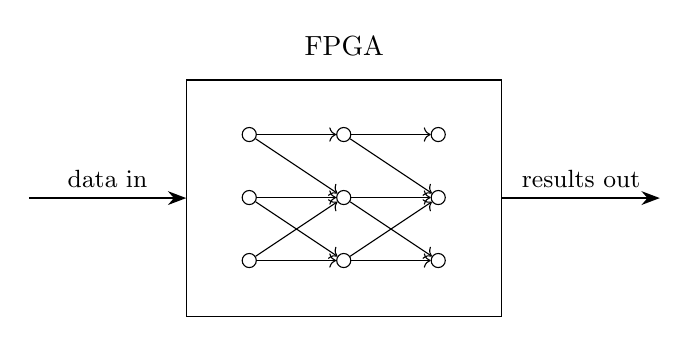
\begin{tikzpicture}[
    block/.style={rectangle, draw, minimum width=4cm, minimum height=3cm, align=center},
    arrow/.style={-{Stealth}, thick},
    nodecircle/.style={circle, draw, fill=white, inner sep=1.8pt},
    textnode/.style={font=\small}
    ]

    % FPGA block
    \node[block] (fpga) {};
    \node[above=5pt of fpga.north] {FPGA};

    % Input and output coordinates
    \coordinate[left=2cm of fpga.west] (datain);
    \coordinate[right=2cm of fpga.east] (resultsout);

    % Data in and results out arrows
    \draw[arrow] (datain) -- (fpga.west) node[midway, above, textnode] {data in};
    \draw[arrow] (fpga.east) -- (resultsout) node[midway, above, textnode] {results out};

    % Define circle positions inside FPGA block in 3 vertical layers
    \foreach \layer/\x in {1/0.8, 2/2.0, 3/3.2} {
        \foreach \row/\y in {1/0.7, 2/1.5, 3/2.3} {
            \node[nodecircle] (c\layer\row) at ([shift={(\x cm,-\y cm)}]fpga.north west) {};
          }
      }

    % Arrows from layer 1 to layer 2 (mixed connections)
    \draw[->] (c11) -- (c21);
    \draw[->] (c11) -- (c22);
    \draw[->] (c12) -- (c22);
    \draw[->] (c12) -- (c23);
    \draw[->] (c13) -- (c22);
    \draw[->] (c13) -- (c23);

    % Arrows from layer 2 to layer 3 (mixed connections)
    \draw[->] (c21) -- (c31);
    \draw[->] (c21) -- (c32);
    \draw[->] (c22) -- (c32);
    \draw[->] (c22) -- (c33);
    \draw[->] (c23) -- (c32);
    \draw[->] (c23) -- (c33);

  \end{tikzpicture}
  \caption{Lack of latency overhead of an FPGA inference stream}
  \label{fig:fpgadiagram}
\end{figure}

\section{Model Architectures and Considerations}
Achieving real time hyperspectral image processing requires not just efficient hardware design, but also consideration of the model architectures that will work most effectively on an FPGA. Because of our control over hardware\mycomment{Note: not sure what I wanted to say here and usage of pipelining and fixed data types},
we might be able to achieve latency improvements at the marginal expense of model accuracy. Furthermore, we can't rely on conventional wisdom regarding runtime on a GPU and we aren't concerned about the training time of our model. We can accept an excessively long model training time if it results in inference runtime improvement since the true bottleneck to the success of the project is inference latency. In comparison, training time is largely irrelevant and can be done with many more resources without issue.
% If this isn't clear in the paper, I should make it clear that we are able to train on GPUs with no problem

It is also necessary to consider the memory usage of our model. A convolutional neural network (CNN) that needs to store a large amount of data in DRAM for its kernel passthrough because of the limited amount of local FPGA memory is inefficient because of the latency involved in storing and accessing that data. We could attempt to pipeline data from DRAM in such a way that there is no latency overhead involved in accessing it, but this adds additional complexity to our hardware design and implementation. Thus we would like to design and use a model that is fast, accurate, small, and leverages the computational advantages of a programmable circuit.

\section{Kolmogorov-Arnold Networks}
A Kolmorgorov-Arnold Network (KAN) is a type of neural network that directly learns nonlinear activation functions between each layer of the network rather than learning weights for linear transformations and applying a fixed nonlinear activation function between each layer \cite{kan}.

\begin{figure}[H]
  \centering
  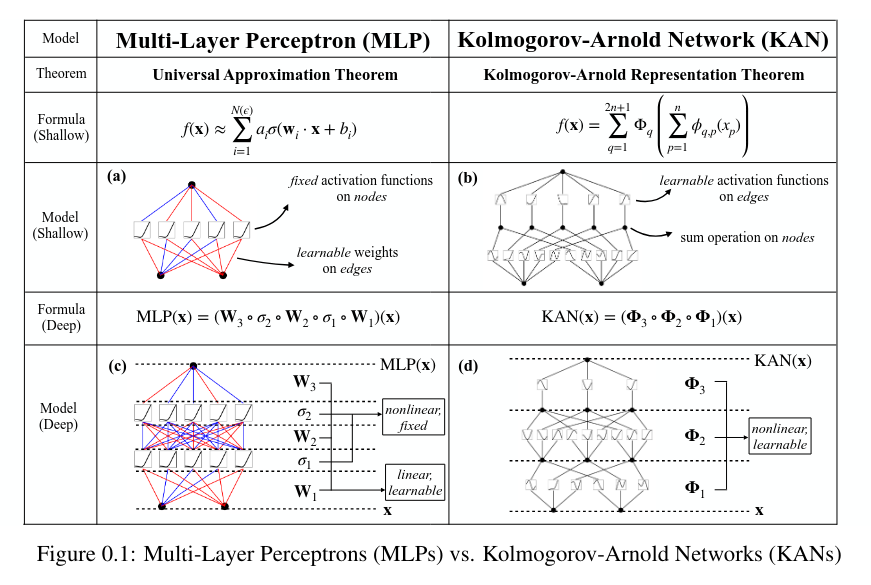
\includegraphics[scale=0.5]{mlpkan.png}
  \caption{A visualization of the differences between a KAN and traditional MLP \cite{kan}}
\end{figure}

KANs generally perform similarly to multilayer-perceptron networks (MLPs) on most tasks; whether they will find widespread use is still largely unknown given their recent development in the field of machine learning. However, for us they have an extremely appealing property: we can achieve performance improvements by encoding their nonlinear functions as lookup tables within the fabric of our FPGA. What this means is that for a given nonlinear function over some fixed domain (this domain is determined based on the inputs the function sees during training -- thus it shifts to properly accommodate incoming data), we can choose some granularity for a mesh, calculate outputs across that mesh, and then store those results in a lookup table. Then for some input, we can interpolate between the entries of our lookup table to determine an approximate result. Because the KAN is composed entirely of nonlinear activation functions, this extremely fast lookup process encompasses the entirety of model inference, potentially granting significant speed improvements within the fabric of our FPGA.

\begin{figure}[H]
  % No centering because the label naturally pushes to the right
  % \centering
  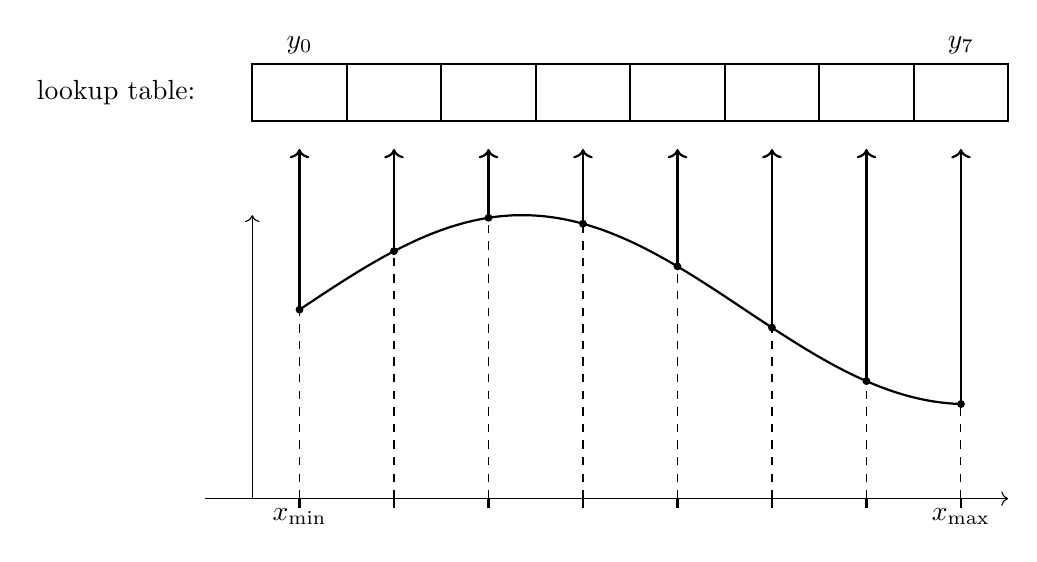
\begin{tikzpicture}[scale=1.2]

    % Parameters
    \def\npoints{8}
    \def\tableHeight{4}
    \def\boxWidth{1}
    \def\xstart{1} % Starting x-value (instead of 0)
    \def\xend{8}   % 8 intervals = 9 points

    % Axes
    \draw[->] (\xstart - 1, 0) -- (\xend + 0.5, 0); % x-axis
    \draw[->] (\xstart - 0.5, 0) -- (\xstart - 0.5, 3); % y-axis

    % Function and evaluation points
    \foreach \i in {0,...,7} {
        \pgfmathsetmacro\x{\xstart + \i}
        \pgfmathsetmacro\y{2 + sin(deg((\x - 1)/1.5))} % offset for natural xmin
        \filldraw[black] (\x,\y) circle (1pt);  % function evaluation point
        \draw[dashed] (\x,0) -- (\x,\y);       % dashed vertical line
        \draw[->, thick] (\x,\y) -- (\x,\tableHeight - 0.3); % arrow to table
        \draw[thick] (\x,0) -- ++(0,-0.1);     % x-axis tick mark
      }

    % Draw the function curve
    \draw[thick, smooth, domain=\xstart:\xend, samples=100]
    plot(\x, {2 + sin(deg((\x - 1)/1.5))});

    % Lookup table boxes (aligned with center of evaluation points)
    \foreach \i in {0,...,7} {
        \pgfmathsetmacro\x{\xstart + \i - 0.5}
        \draw[thick] (\x, \tableHeight) rectangle ++(\boxWidth, 0.6);
      }

    % Labels
    \node[below] at (\xstart, 0) {$x_{\min}$};
    \node[below] at (\xend, 0) {$x_{\max}$};
    \node[above] at (\xstart + 0.0, \tableHeight + 0.6) {$y_0$};
    \node[above] at (\xend - 0.0, \tableHeight + 0.6) {$y_7$};
    \node[left] at (\xstart - 1, \tableHeight + 0.3) {lookup table:};
  \end{tikzpicture}
  \caption{An example 8 entry lookup table over a nonlinear function}
  \label{fig:lkup-diagram}
\end{figure}

\subsection{Lookup Tables in an FPGA}
In general, the lookup tables for a KAN require a significant amount of memory. For a fully connected KAN consisting of 5 layers and 200, 32, 32, 32, and 16 nodes within each layer respectively, there will be $(200 * 32) + (32 * 32) + (32 * 32) + (32 * 16) = 8960$ lookup tables. If each has a fine mesh of 4096 entries and each entry is 4 bytes, then simply storing the entries of each lookup tables would take $8960 * 4096 * 4 \text{ bytes} \approx 147 \text{ Mb}$. In reality, the lookup tables for each layer need not be loaded at the same time. Also, the fixed point types we use will almost certainly be less than $4$ bytes, and we can experiment with table granulatities of less than $4096$ and see how it affects accuracy. It nevertheless remains true that the memory overhead of lookup tables is significant. Thus it is necessary to write a Linux device driver that can efficiently load lookup table values from DRAM into static fabric memory (SRAM) so that they can be used by our FPGA.
% Do I want to elaborate on this driver and its necessary capabilities, what it would do, why it's important? Almost certainly yes, but perhaps when I know a little bit more about it. Also could consider doing it elsewhere

% -----------------------------------------------------------------------------------------------------------------------------------

% \section{Project Work}

\section{CNN Implementation and Benchmarking}
At the start of the project, it was important to do performance benchmarking on existing hyperspectral vision models in order to calibrate our expectations of the kind of workload we would encounter when doing real-time inference. We used a previous paper and model created by researchers at Montana State University as our CNN benchmark \cite{Morales_2021} \cite{rs13183649}. Their code uses binning and many convolutional layers to classify pixels of the well-known Indian Pines Dataset. The structure of their model is shown in \autoref{fig:cnn-struct}

\begin{figure}[H]
  \centering
  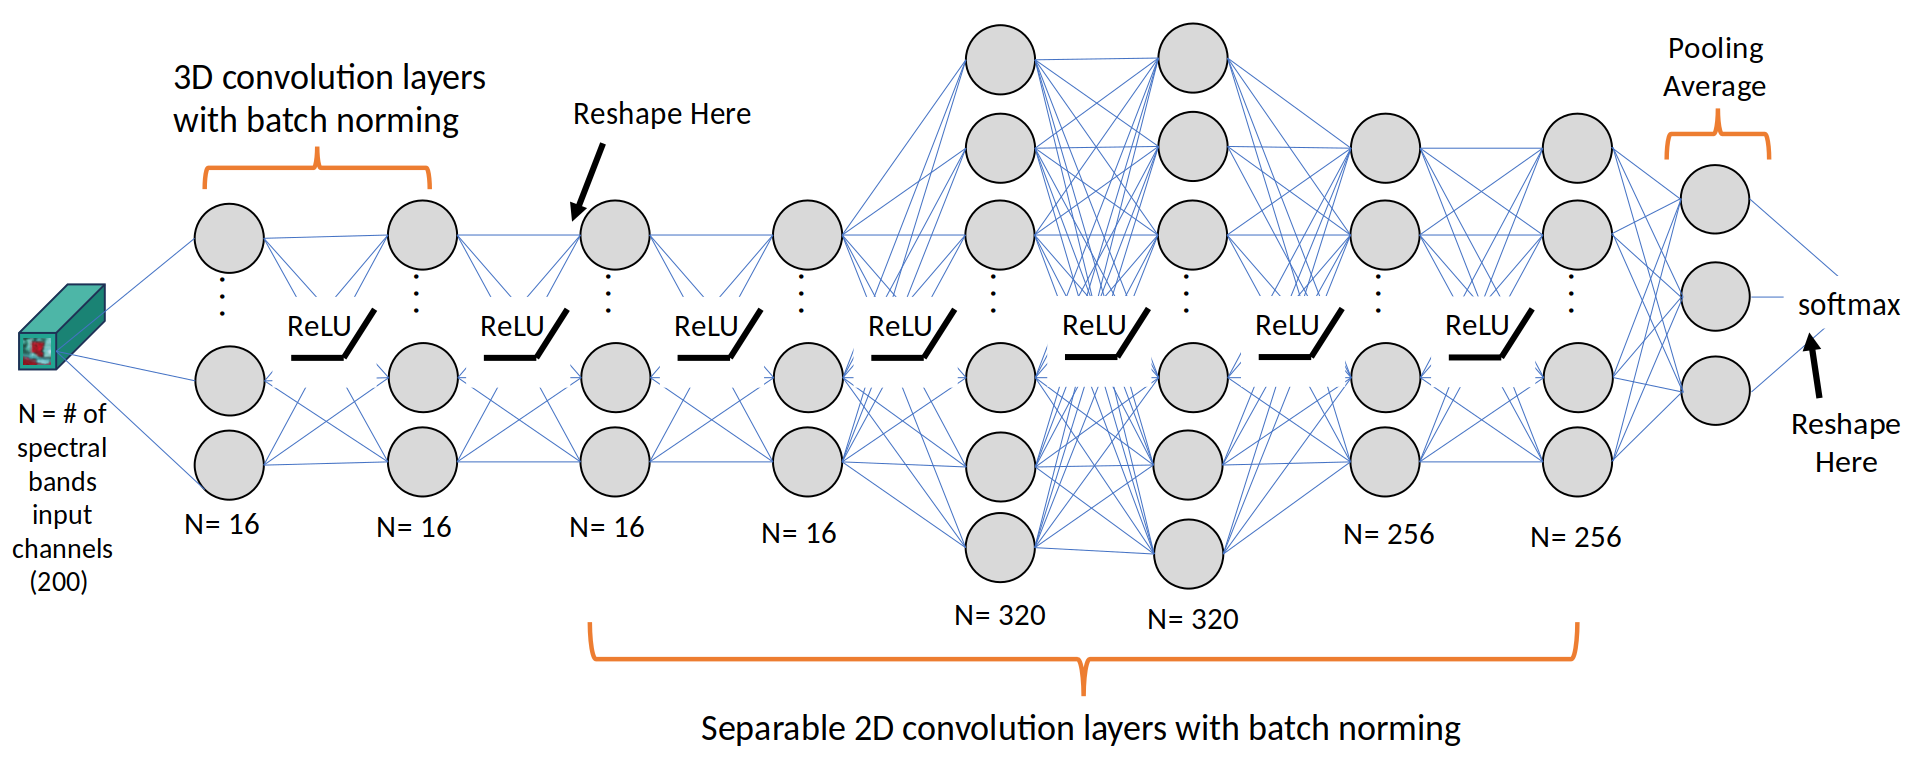
\includegraphics[scale=0.25]{cnn_arch.png}
  \caption{Visualization of the CNN model \cite{dirk-presentation}}
  \label{fig:cnn-struct}
\end{figure}

I recreated their code faithfully in C. My goal was to get a sense of the number of operations involved in a large convolutional network as well as to allow benchmarking directly on the CPU/GPU of our board. \mycomment{It should be noted that this program naturally ran very slowly compared to the Python code due to the lack of optimizations that pytorch implements such as GPU acceleration, parallelism, memory optimization, operator fusion, and more.}The CNN model did about 2 billion elementary add and multiply operations for each pixel it classified.\\\\
\textbf{The operations involved in a forward pass of the CNN:}
\begin{lstlisting}[language=python]
self.conv_layer1 = nn.Sequential(
    nn.Conv3d(in_channels=img_shape[0], out_channels=16, kernel_size=3, padding=1),
    nn.ReLU(),
    nn.BatchNorm3d(16))

self.conv_layer2 = nn.Sequential(
    nn.Conv3d(in_channels=16, out_channels=16, kernel_size=3, padding=1),
    nn.ReLU(),
    nn.BatchNorm3d(16))

self.sepconv1 = nn.Sequential(
    nn.Conv2d(in_channels=16 * img_shape[1], out_channels=16 * img_shape[1], kernel_size=5, padding=2, groups=16 * img_shape[1]),
    nn.ReLU(),
    nn.Conv2d(in_channels=16 * img_shape[1], out_channels=320, kernel_size=1, padding=0),
    nn.ReLU(),
    nn.BatchNorm2d(320))

self.sepconv2 = nn.Sequential(
    nn.Conv2d(in_channels=320, out_channels=320, kernel_size=3, padding=1, stride=stride, groups=320),
    nn.ReLU(),
    nn.Conv2d(in_channels=320, out_channels=256, kernel_size=1, padding=0),
    nn.ReLU(),
    nn.BatchNorm2d(256))

self.sepconv3 = nn.Sequential(
    nn.Conv2d(in_channels=256, out_channels=256, kernel_size=3, padding=1, stride=stride, groups=256),
    nn.ReLU(),
    nn.Conv2d(in_channels=256, out_channels=256, kernel_size=1, padding=0),
    nn.ReLU(),
    nn.BatchNorm2d(256))

self.average = nn.AvgPool2d(kernel_size=out)

if classes == 2:
    self.fc1 = nn.Linear(256, 1)
else:
    self.fc1 = nn.Linear(256, self.classes)
\end{lstlisting}

\begin{lstlisting}[language=python]
def forward(self, x):
    # 3D Feature extractor
    x = self.conv_layer1(x)
    x = self.conv_layer2(x)

    # Reshape 3D-2D
    x = reshape(x, (x.shape[0], self.img_shape[1] * 16, self.img_shape[2], self.img_shape[3]))

    # 2D Spatial encoder
    x = self.sepconv1(x)
    x = self.sepconv2(x)
    x = self.sepconv3(x)

    # Global Average Pooling
    x = self.average(x)

    x = reshape(x, (x.shape[0], x.shape[1]))
    x = self.fc1(x)
    return x

\end{lstlisting}

\section{KAN Implementation and Benchmarking}
\subsection{Design}
I likewise implemented a KAN model in C that performed pixel-wise classification on the Indian Pines dataset. The layers of the model consisted of 200, 32, 32, 32, 16 nodes respectively. I implemented the model as closely as possible to how it would be done in fabric; this means that I used lookup tables to approximate nonlinear functions and adder trees to store values and perform addition. I used CFFI (C Foreign Function Interface) to create a shared C library that can be called from Python to more easily facilitate populating the lookup tables and experimenting with different model architectures. Thus a model can be trained in Python, each nonlinear function can be evaluated at a mesh of points, and we can populate the lookup tables of the C version by calling the appropriate function.

Additionally, because the final FPGA implementation will use fixed data types which operate as binary representations of a decimal number, I implemented scaling as a compile-time option so that the lookup tables can be populated with scaled values in the range $[0,1]$ and rescaled outwards. This will save space and complexity in the fabric implementation by ensuring we know that the implicit decimal point of our fixed data type always exists on the far left side of its representation.

\subsection{Lookup Table Implementation}
Each lookup table consists of both the actual stored values as well as the meta-data necessary to rescale our output (if scaling is enabled).

\begin{lstlisting}[language=C]
struct lkup_tbl {
    float tbl[TBL_SIZE];
    float xmin;              // x val associated with table[0]
    float xmax;              // x val associated with table[TBL_SIZE - 1]
    float xdist;             // dist between x values 
                             // xdist = (xmax - xmin) / TBL_SIZE
    float inv_xdist;         // the reciprocal of xdist for division
    float ymin;
    float ymax;
};
\end{lstlisting}

Thus to do a lookup on our table, we use \texttt{xmin}, \texttt{xmax}, \texttt{xdist}, and \texttt{inv\_xdist} to do linear interpolation between the lookup table entries nearest to our input. Note that \texttt{inv\_xdist} exists only because the division operation is expensive in fabric, so it is better to precompute it.

\begin{lstlisting}[language=C]
static float lookup(float x, struct lkup_tbl *table) {
    if (x <= table->xmin) {
        return table->tbl[0];
    }
    else if (x >= table->xmax) {
        return table->tbl[TBL_SIZE - 1];
    }
    float idxf = (x - table->xmin) * table->inv_xdist;
    // remainder is now the proportion that x is between idx and idx + 1
    float remainder = fmodf(idxf, 1);
    assert(remainder >= 0);

    int idx = (int) idxf;
    return table->tbl[idx] + ((table->tbl[idx + 1] - table->tbl[idx]) * remainder);
}
\end{lstlisting}

Each node of our model contains a lookup table for every node in the next layer as well as a single adder tree. An adder tree is a collection of values that are stored so that they can be added together in parallel by multiple processors. A layer is a collection of nodes; when we propogate from one layer to another, for each node in our layer we first accumulate the existing values of our adder tree. Then for each lookup table corresponding to a node in the next layer, we find the output based on our accumulated value and place it in the adder tree for that node. This process is fully demonstrated in the following two algorithms, which show a complete neural network forward pass implemented with lookup tables.

\begin{algorithm}[H]
  \caption{Forward Algorithm}
  \label{alg:forward}
  \begin{algorithmic}[1]
    \Function{Forward}{$\text{model}, \text{input}$}
    \State $\Call{InitVals}{\text{model}.\text{layers}[0], \text{input}}$
    \For{$i = 0$ \textbf{to} $\text{model}.\text{len} - 2$}
    \State $\Call{Propagate}{\text{model}.\text{layers}[i]}$
    \EndFor
    \State $\text{ret} \gets []$
    \State $\text{final\_layer} \gets \text{model}.\text{layers}[\text{model}.\text{len} - 1]$
    \ForAll{$\text{node} \in \text{final\_layer}$}
    \State $\text{node}.\text{val} \gets \Call{Accumulate}{\text{node}.\text{adder\_tree}}$
    \State $\text{ret}.\Call{Append}{\text{node}.\text{val}}$
    \EndFor
    \State \Return $\text{ret}$
    \EndFunction
  \end{algorithmic}
\end{algorithm}

\begin{algorithm}[H]
  \caption{Propagation Algorithm}
  \label{alg:propagate}
  \begin{algorithmic}[1]
    \Require $\text{layer}$ is not the final layer of the model
    \Statex \textit{This algorithm operates without scaling and assumes the model is fully connected}
    \Function{Propagate}{$\text{layer}$}
    \ForAll{$\text{node} \in \text{layer}$}
    \State \textit{No need to accumulate first layer -- inputs are already in node.val}
    \If{$\text{layer}.\text{idx} \ne 0$}
    \State $\text{node}.\text{val} \gets \Call{Accumulate}{\text{node}.\text{adder\_tree}}$
    \EndIf
    \For{$j = 0$ \textbf{to} $\text{node}.\text{next\_layer}.\text{len} - 1$}
    \State $\text{lookup\_table} \gets \text{node}.\text{tables}[j]$
    \State $\text{target\_node} \gets \text{node}.\text{next\_layer}.\text{nodes}[j]$
    \State $\text{target\_tree} \gets \text{target\_node}.\text{adder\_tree}$
    \State $\text{output} \gets \Call{Lookup}{\text{node}.\text{val}, \text{lookup\_table}}$
    \State $\text{target\_tree}.\text{inputs}[\text{target\_tree}.\text{ptr}] \gets \text{output}$
    \State $\text{target\_tree}.\text{ptr} \gets \text{target\_tree}.\text{ptr} + 1$
    \EndFor
    \EndFor
    \EndFunction
  \end{algorithmic}
\end{algorithm}


\subsection{Accuracy Loss and Performance}
For a single sample, the forward function with a lookup table size of 4096 takes 0.00085-0.00087 seconds to run in C with my CPU: 12th Gen Intel(R) Core(TM) i7-1260P (16) @ 4.70 GHz. The final results vary by 0.1 - 0.01 from the actual Python results which generally should not be enough to change the pixel classification, proving the viability of a KAN lookup table implementation.

% Cursory proofreading complete up to this point
\section{Device Driver Development}

\subsection{Motivation}
% Note: edit this after actual implementation
While it is necessary to transfer large amounts of data to static fabric memory (SRAM) to populate KAN lookup tables, this memory is not typically accessible to a user. Thus, it is necessary to create a Linux device driver that can transfer memory from DRAM to the FPGA. In particular, my goal was to create a block driver which could write blocks of memory to SRAM\mycomment{This is not even what I ended up writing lol}. This would allow an easy interface between the userspace of our system and the SRAM of our fabric. Because of the large memory demand of lookup tables, it will be necessary to load and unload multiple sets of lookup tables in the course of the classification of a single pixel. Thus an interface between user and FPGA memory is especially important for any KAN implementation.
% in for our lookup table implementation, which uses large amounts of memory which needs to be loaded and unloaded frequently into fabric memory.
% Our FPGA contains two seperate ports

\subsection{Board and Development Environment Setup}
I used a Kria KV260 board for my driver development and testing. Information and instructions on the board setup process can be found \href{https://github.com/night1rider/Xilinx-KR260-Intro/blob/Hello-World/Documentation/00_hello_world_kr260.md}{here} \cite{board-setup}. This involved using Petalinux to generate a custom kernel for my board and installing an Ubuntu root filesystem so I would have access to packages and a more typical development environment. I also set up networking servers between my virtual machine and device to streamline the development process.

\subsection{Background Information and Driver Design}
It is important to distinguish between a computer's address space and its actual physical memory. While the KV260 board has only 4 GB of DRAM, it has a 40 bit address space (typical for a 64 bit CPU), which spans about a terabyte. This means that large swaths of the address space are reserved for data buses and peripheral devices. Thus while a user might typically only write to physical memory, they can interact with a device driver to write to a specific address and span of the address space that corresponds to a data bus accessible to our FPGA.

A device tree in Linux describes the hardware that Linux is running on so that the kernel can be aware of the components it needs to manage.

The 224 GB region from \texttt{0x0010\_0000\_0000} to \texttt{0x0047\_FFFF\_FFFF} corresponds to the AXI bus \texttt{M\_AXI\_HPM0\_FPD} which is accessible to our FPGA \cite{zynq-doc}. Inside of our device tree we can create two new entries, one at the base address of \texttt{0x0010\_0000\_0000} and the other at the base address of \texttt{0x0030\_0000\_0000}, each with a span of 16 KB. Then by attaching our drivers to these entries, they will read and write from these addresses. The AXI bus connects to two seperate ports in the static RAM of the FPGA. We can distinguish between the two ports on the basis of the addresses of our drivers, thus our first address will write to port A and the second to port B. However, both of these ports connect to the same region of SRAM memory, so a user can write to driver A and read from driver B and recover the same result. This design is illustrated in \autoref{fig:design-fig}.


% Ugly ahh figure
\begin{figure}[H]
  \centering
  \resizebox{1\textwidth}{!}{%
    \scalebox{0.1} {
      \begin{circuitikz}
        \tikzstyle{every node}=[font=\normalsize]
        \draw  (2,11.5) rectangle (4,10.5);
        \draw  (5,12.5) rectangle (7,11.5);
        \draw  (5,10.5) rectangle (7,9.5);
        \draw [->, >=Stealth] (4,11) -- (5,12);
        \draw [->, >=Stealth] (4,11) -- (5,10);
        \node [font=\normalsize] at (3,11) {User};
        \node [font=\normalsize] at (6,12) {Driver B};
        \node [font=\normalsize] at (6,10) {Driver A};
        \draw  (9,14.5) rectangle (10.75,6.25);
        \draw [short] (9,12) -- (10.75,12);
        \draw [short] (9,9.25) -- (10.75,9.25);
        \draw [->, >=Stealth] (7,12) -- (9,10.75);
        \draw [->, >=Stealth] (7,10) -- (9,9.25);
        \draw [dashed] (9,10.75) -- (10.75,10.75);
        \draw [short] (11.5,12) -- (11.5,7.75);
        \draw [short] (11.25,9.25) -- (11.75,9.25);
        \draw [short] (11.25,12) -- (11.75,12);
        \draw [->, >=Stealth] (11.5,7.75) -- (14.5,7.75);
        \draw  (15.5,8.5) rectangle (16.75,6.25);
        \draw [<->, >=Stealth] (14.5,7.75) -- (15.5,7.75);
        \draw [dashed] (15.5,7.75) -- (16.75,7.75);
        \draw [dashed] (15.5,7) -- (16.75,7);
        \node [font=\normalsize] at (10,15.25) {Physical Address Space};
        \node [font=\normalsize] at (16,8.75) {SRAM};
        \node [font=\tiny] at (13,12) {0x0047\_FFFF\_FFFF};
        \node [font=\tiny] at (13,10.75) {$0x0030\_0000\_0000$};
        \node [font=\tiny] at (13,9.25) {0x0010\_0000\_0000};
        \node [font=\normalsize] at (12.5,14.5) {0x0100\_0000\_0000};
        \node [font=\normalsize] at (11.25,6.25) {0x0};
        \node [font=\normalsize] at (15,8) {A/B};
        \node [font=\small] at (12.5,7.5) {M\_AXI\_HPM0\_FPD};
      \end{circuitikz}
    }
  }%

  \caption{The design of our device driver}
  \label{fig:design-fig}
\end{figure}

\subsection{Driver Implementation} % Probably want to split this up somehow
% Talk about the dual port design, axi bus, etc.
% I chose to test the ability of our driver to connect to the dual-port in the fabric by constructing two seperate device tree entries at fixed addresses of \texttt{0x10\_0000\_0000} and \texttt{0x30\_0000\_0000} in the reserved region of \texttt{M\_AXI\_HPM0\_FPD} with a span of 16 KB each. The plan was to connect a seperate driver to each of these entries and test their ability to read the data that the other wrote to the shared portion of FPGA memory.

I began the process of implementing my driver by creating a design for the fabric of our FPGA which connected \texttt{M\_AXI\_HPM0\_FPD} to two \texttt{AXI BRAM Controllers} at fixed addresses and ranges that correspond to our device tree entries. I then connected each of these \texttt{AXI BRAM Controllers} to seperate ports in the \texttt{Block Memory Generator}. For a visualization of this simplistic design, refer to \autoref{fig:fpga-design}.

\begin{figure}[H]
    \centering
    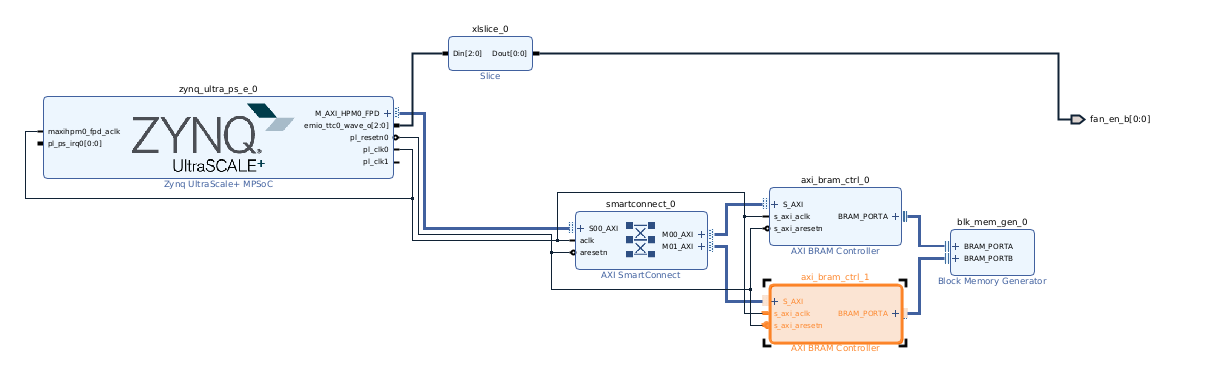
\includegraphics[scale=0.5]{fpga_prog_img.png}
    \caption{The dual port fabric design of our FPGA}
    \label{fig:fpga-design}
\end{figure}

I designed a platform device driver which is intended to connect to non-discoverable hardware and peripherals that require manual registration in Linux. I combined this with the the Block-IO (bio) API used to handle reading and writing in block drivers.

When testing my driver, I discovered that reading and writing would not work properly past the first 64 bits of our request. I learned that the reason for this is because some of our hardware organizes memory as 64 bit lines, and so reading and writing wouldn't work properly beyond that range. Thus an attempt should be made to resolve this hardware issue so that block IO can work properly, and if this turns out to be impossible, then the driver should be modified to be a character driver. A character driver does IO on only a single register at a time and operates sequentially. Nevertheless, ignoring these hardware limitations, the driver worked properly and effectively when tested. 

% -----------------------------------------------------------------------------------------------------------------------------------

\section{Future Work}
\subsection{KAN Accuracy Testing}
Currently the KAN lookup table implementation accommodates toggling scaling and changing the lookup table sizes at compilation time of the shared library. However, it does not currently accommodate changing data type precision or using fixed data types as would occur in fabric. It would be useful to implement this in some fashion. Additionally, it will be necessary and useful to do parameter sweeps over lookup table size and data type precision to see what the accuracy tradeoffs are for various model sizes. Shrinking these two parameters would mean that we can shrink the amount of memory that our model will need to load into SRAM, making our final implementation easier to create and more efficient

\subsection{Model Pruning}
Given the importance of a small and efficient model for our inference speed, there may be additional opportunities to decrease the size of an already trained KAN model. In particular, if some of our nonlinear functions are similar enough to each other, we might be able to cluster together their computation in order to avoid unnecessary lookup table loading. Also, if any of our functions appear to be roughly linear, then that could be an indication that our model is too large and the functions are unnecessary for our inference process. The KAN Python library already contains an API for pruning its models, but previous work on our project did not have much success at using it. It is possible that this was partially attributable to peculiar model hyperparameter choices that made the nonlinear functions relatively extreme. Further exploration, or an approach that utilizes other methods such as K-means clustering, should be considered to see if they can further reduce model size.

\subsection{Modifying the Device Driver}
As I mentioned before, it will be necessary to investigate whether the hardware incompatibility that makes the block IO of our device driver fail is resolvable. If it is not, it will be necessary to convert the driver to be a character driver which does IO on only a single register at a time. This modification should be relatively quick and painless. I would have completed it myself if not for the temporal limitations of the project.

\subsection{Device Driver Overhead}
I did not have time this summer to do testing on the latency overhead of the device driver or the feasibility of loading and unloading lookup tables many times in the course of the classification of a single pixel. If such loading or unloading has a high latency associated with it and needs to be done frequently enough that it makes efficient pipelining of our data difficult, then it may be best to propogate our data in batches instead of as single pixels, caching the intermediate values. This would allow us to perform computations on multiple pieces of data with a single set of lookup tables before loading the next set to continue the computation. This should be considered in the future, especially once we have a better sense of the efficiency of our driver, size of our model and stored data, and difficulty of pipelining the loading `just in time'.

\subsection{Benchingmarking on the FPGA}
For the sake of the project's final paper, it would be useful to benchmark our CNN and KAN C implementations on the CPU/GPU of our board to compare it with the performance of the fabric implementation.

\subsection{Direct Memory Access Implementation}
Currently our driver implementation relies on the CPU to perform read-and-write operations on our data. During this process, the CPU is fully occupied; this is inefficient given the potential scale of loading and unloading necessary throughout the inference process. An alternative is direct memory access (DMA), which entails the CPU initializing a DMA controller and instructing it to begin a transfer. The DMA controller then independently manages the data tracking and communication with the device until the process completes, at which point it provides an interrupt to the CPU. The project's final implementation will likely use DMA if the data transfer process is too strenuous for the CPU alone to perform.
%It should be noted that this is not an entire solution to the device driver overhead discussed above. Similar problems of transfer latency that might motivate more advanced pipelining strategies could still exist even in a DMA implementation. % Sus final couple sentences.

\section{Conclusion}

In conclusion, I began this project by investigating and benchmarking various model architectures that could grant performance improvements in an FPGA implementation. I discovered that the nonlinear functions that comprise a Kolmogorov-Arnold network could be efficiently approximated without a large decrease in accuracy, but that such a representation requires a large amount of data to be stored in the form of lookup tables. To this end, I worked on developing a device driver for our board that would be capable of loading data to the static RAM of our FPGA. The driver was properly written but did not work as expected due to hardware limitations. Nevertheless, it provides a framework for translation into a character driver if the hardware issues are unresolvable, which should be a simple and straightforward process.


\section{Acknowledgements}
I would like to acknowledge my PI Ross Snider for the direction and assistance he has provided on the project. I would also like to thank Nat Sweeney, Zackery Backman, and Dirk Kaiser for the work that they have done and continue to do on the project. Finally I would like to thank my fellow REU members for the support and encouragement they have provided throughout the summer and Isabel Garcia for reading and reviewing this report.

This material is based upon work supported by the National Science Foundation under Grant No. 2349091.

\newpage
% \section{References}
\nocite{*}
\bibliographystyle{IEEEtran}
\bibliography{reference.bib}

\end{document}

